% Chapter Template

\chapter{Conclusion} % Main chapter title

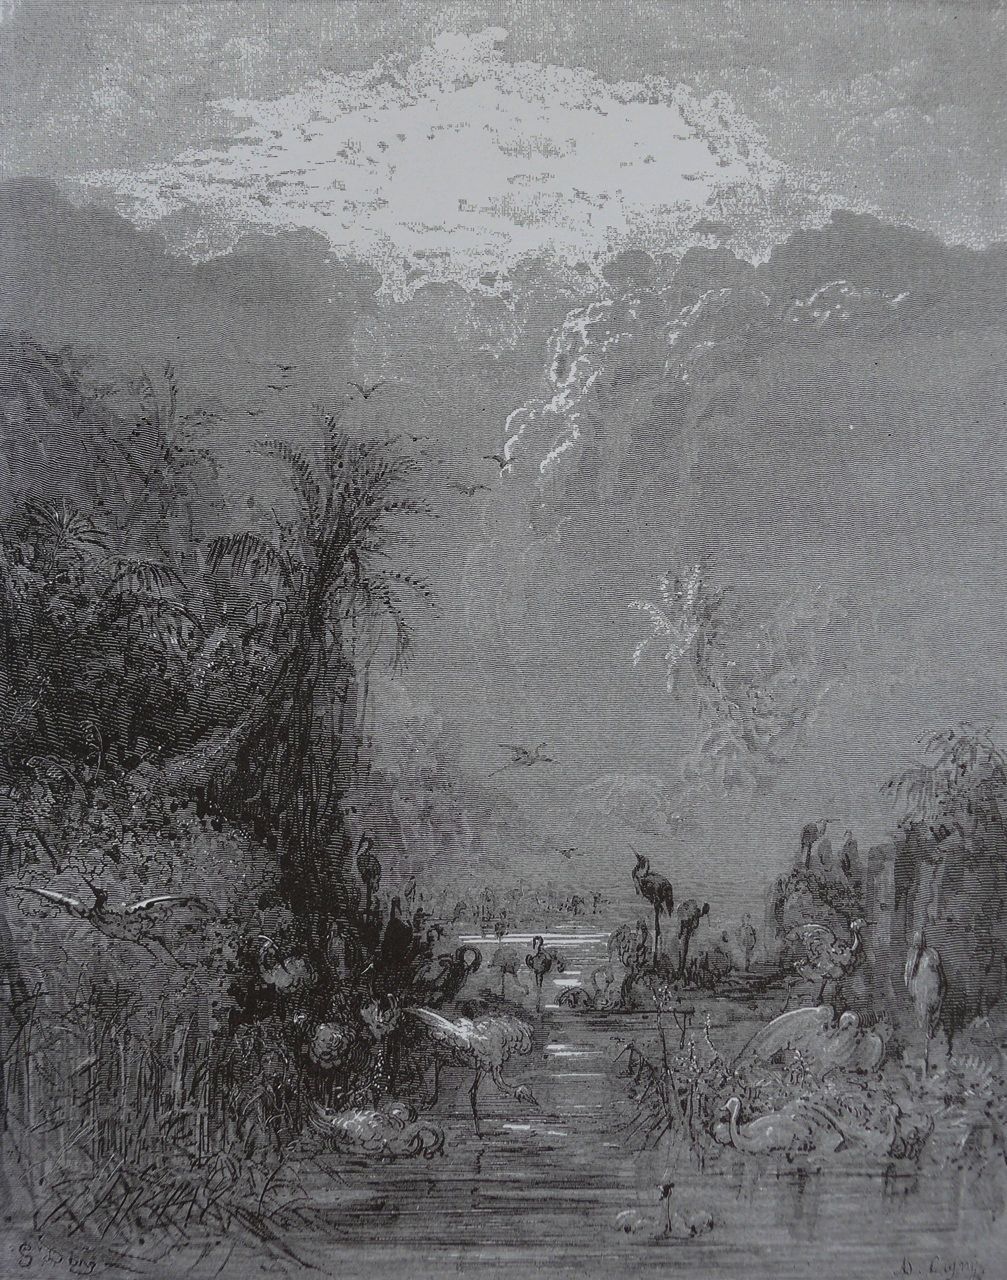
\includegraphics[width=\linewidth,trim={0 4cm 0 15cm},clip]{Paradise_Lost_33}

\label{Chapter 8} % Change X to a consecutive number; for referencing this chapter elsewhere, use \ref{ChapterX}

\section{Overview}

This final chapter will begin by going over the project as a whole and what was achieved during it. Then it will provide an evaluation against the motivation of the project to determine if what was achieved was in line with the aims. Finally, the research questions will be answered.

%----------------------------------------------------------------------------------------
%	SECTION 1
%----------------------------------------------------------------------------------------

\section{Paradise Restored?}

\label{Ch8 Sec1}

Using the techniques described in chapter \ref{Chapter 4}, chapter \ref{Chapter 5} and chapter \ref{Chapter 6}, the MEGA65 project was made more developer friendly, matrix mode was corrected and secure compartmentilization was almost entirely implemented. New developers for the project are now able to more easily build and develop the MEGA65 through the use of a single make file. The MEGA65 is now able to successfully enter and exit matrix mode without disabling any functionality of the rest of the phone. In addition, all of the visual issues in matrix mode have been eliminated. The secure mode hypervisor trap has been implemented as well as some of the secure mode saving. The accpeting and rejecting of a secure container has also been partially implemented and the CPU halting a resuming has been fully implemented.\\

To truely restore paradise the following need to be implemented:
\begin{itemize}
\item{Matrix mode entering and exiting needs to be latched}
\item{Matrix mode exiting needs to stop printing to the screen}
\item{Secure mode needs to save and load save states}
\item{Secure mode entry needs to erase the RAM, ROM and io registers}
\item{Secure mode entry needs to support rejecting entry to a secure container}
\item{Secure mode exit needs to erase RAM, ROM and io registers}
\end{itemize}

%----------------------------------------------------------------------------------------
%	SECTION 2
%----------------------------------------------------------------------------------------

\section{Research Question Answers}

\label{Ch9 Sec2}

\textit{What are the missing or non-functional sub-systems that the MEGA65 requires to be implemented?}\\
The missing and/or non-functional sub-systems of the MEGA65 are:
\begin{itemize}
\item{Save state Saving and Loading}
\item{Secure mode Saving and Loading}
\item{Secure mode ACCEPT and REJECT Implementation}
\item{SD card Read Protection}
\item{CPU Lock Protection}
\item{Matrix mode Key Scanning}
\item{SDXC Compatibility}
\end{itemize}

\textit{How can these sub-systems be implemented?}\\
These sub-systems can be implemented as follows:
\begin{itemize}
\item{Save state Saving and Loading}\\
  The save and load states can be implemented in the place holder files. Since the supporting hardware has already been developed, all that is required is the assembly implementations.\\
\item{Secure mode Saving and Loading}\\
  The secure mode saving and loading require the implementation of the save state functions. Additionally, they require some of their own assembly code. This code is required in the hypervisor traps and, like the save states, already has the supporting hardware around it.\\
\item{Secure mode "ACCEPT" and "REJECT" Implementation}\\
  Much like the previous two points, the accepting and rejecting functionality only requires the software implementation.\\
\item{SD card Read Protection}\\
  This can be simply implemented through manipulation of the SD card software. Enabling a software SD card check can be done by reading the partition table and if it is corrupted, disallowing all further writes and reads. In hardware, a similar check could possibly be done, this depends on the functionality of the SD card controller.\\
\item{CPU Lock Protection}\\
  In order to prevent accidental locking of the CPU, matrix mode could be tied to the halting and resuming of the CPU.\\
\item{Matrix mode Key Scanning}\\
  The matrix mode key scanning can be implemented by implementing a working latch for the enter and exit key combinations. This latch should cause the iomapper to ignore the held version of these key combinations.\\
\item{SDXC Compatibility}\\
  Adding SDXC support, such as reset, read and write protocols, to the existing SD card hardware would enable this functionality.\\ 
\end{itemize}

\textit{How can the simplicity, understandability and hence, the security of these sub-systems be maximised?}\\
By implementing the sub-systems in accordance with the UNIX philosophy of "Do one thing and do it well.", it was possible to create highly understandable and secure units that are able to make up the whole that is the MEGA65
\\
\textit{How can the complete MEGA65 architecture be physically prototyped on the bench?}\\
The complete architecture of the MEGA65 was prototyped via an FPGA. This FPGA contained the all of the MEGA65 architecture and was supplemented by 3rd party hardware, such as the modem.
\\
\textit{How can the secure compartmentalisation's architecture planned for the MEGA65 be realised?}\\
Through a combination of hardware and software the MEGA65's plan for secure compartments can be realised. The hardware can handle the actions that are desired to be atomic, as well as the disabling of data escaping mediums. The software can handle the actions that require user input and that are not atomic.
